%Results
For this paper, we simulated audits for 
the 2020 Presidential election
in all US states whose margin was at least $5\%$.
Round sizes increase roughly proportional to the inverse
square of the margin, so 
smaller margins are computationally much more expensive to simulate.
For each of these states, we simulated 
$10,000=10^4$ audits with the announced
underyling ballot distribution
and an additional $10,000=10^4$ audits with a tie
as the underlying ballot distribution.
These are reasonable choices for inital simulation experiments
because most audits frame the stopping decision as a binary
hypothesis test where the null hypothesis assumes an underyling tie
and the alternative hypothesis assumes the announced distribution.
A standard first round size in ballot-polling audits
has been one which achieves a $90\%$ probability
of stopping, and we chose round sizes to reflect this standard
in our simulations.
We ran our simulations for up to five rounds.
With a $90\%$ stopping probability, 
an audit only has a $a$ probablity of not stopping
by the end of the fifth round, assuming the outcome was correctly
announced.

\subsection{End-of-Round \BRAVO}
For the EoR \BRAVO simulations, our software estimated and used for each round
the minimum round size that would achieve a $90\%$ probability of stopping.
For the simulations with the announced outcome as the underlying
ballot distribution, for each round $j$ we computed the proportion of audits 
that stopped in round $j$ among those that had not stopped before round $j$.

\begin{figure}[H]
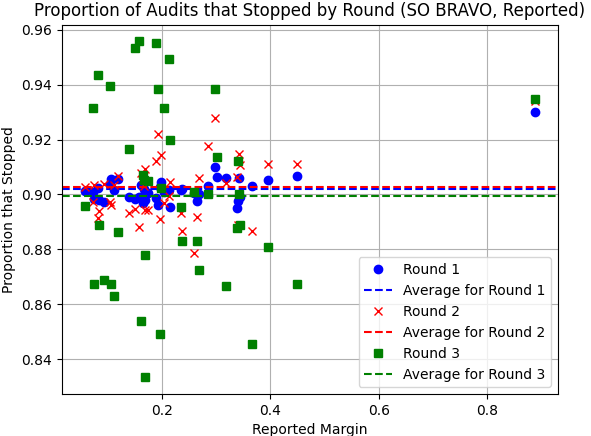
\includegraphics[width=\textwidth]{eor_bravo_90perc_10^4_corrected/sprob_first_three.png}\caption{
For the first three rounds of the EoR \BRAVO simulations, this plot shows the proportion of audits that stopped in the $j$th round
to all audits which had not yet stopped before the $j$th round.}
\label{fig:eor_bravo_sprob}
\end{figure}

In Figure \ref{fig:eor_bravo_sprob}, we display proportions for only the first three rounds
since very few audits, $(.1)^{j-1}\cdot(10^4)$ on average, 
make it to the $jth$ round.
As  a result, the proportions are based on an exponentially smaller dataset in each round.
The proportions shown in Figure \ref{fig:eor_bravo_sprob} give an estimate
of the true probability of an EOR \BRAVO audit stopping in the $j$th round,
given that it has not already stopped in a previous round. 
In \ref{fig:eor_bravo_sprob}, we see that, especially in earlier rounds for which 
the values are more representative of true audit behavior, 
our predictions are accurate.
In particular, the average across all margins is just above $.9=90\%$ for
all three rounds.

The risk of this audit, across all $5$ rounds, is an important metric since it determines whether an audit is risk-limiting.
Therefore, we now consider the proportion of audits that stopped with an underlying tie.
This proportion, for a risk-limiting audit, should approach a value less than the risk limit, $0.1$, as more audits are performed.

\begin{figure}[H]
\includegraphics[width=\textwidth]{eor_bravo_90perc_10^4_corrected/total_risk.png}
\caption{For each state margin, this plot shows
the proportion of EOR \BRAVO audits with an underlying
tie that stopped.}
\label{fig:eor_bravo_risk}
\end{figure}

Figure~\ref{fig:eor_bravo_risk} makes it clear that the risk of EOR \BRAVO is roughly
an order of magnitude less than the risk limit. 
That is, on average, roughly $10$ times more audits could have stopped 
with the audit still meeting the risk limit.
These simulations support the claim made in [\Minerva paper]
that EOR \BRAVO is unnecessarily conservative and thus requires
more ballots on average.

% \subsection{Selection-Ordered BRAVO}
% next_sample_size code is slow... tie simulations running still!

\subsection{\Minerva Simulations}
For \Minerva, it has not been shown that round sizes can be chosen
during the audit. That is, an adversary with knowledge of the history
of the audit may be able to choose round sizes which cause the 
risk of the audit to exceed the risk limit.
For this reason, we have to choose the round sizes of a \Minerva 
audit a priori.
For this paper, we consider two choices of round sizes.
For both, we estimate and then use the minimum first round size 
which achieves
a $90\%$ probability of stopping.
Then, for subsequent rounds, we either (i) 
draw the same number of ballots in each round or (ii)
multiply the previous round size by a factor of $1.5$ and 
sample this many new ballots.
We consider the case of drawing samples of the same size
because it may reflect a practical way to continue an
audit; if election officials have selected some first round size within
reasonable logistical bounds, drawing the same number of 
ballots in subsequent rounds may be practical.
We also consider round sizes with samples increasing by a multiple
of $1.5$ because this multiple gives a very rough approximation of 
round sizes with a $90\%$ probability of stopping.

\subsubsection{Round Sizes with Multiple of $1.0$}

As with the preceding simulations, we ran $10,000=10^4$ trials
per state for both the underlying tie and underlying reported
outcome.

\begin{figure}[H]
\includegraphics[width=\textwidth]{minerva_multiround_1x_10^4/total_risk.png}
\caption{This plot shows, for each state's margin, the proportion of audits that stopped of
all $10^4$ audits with an underlying tie in the simulations with a round size multiple of $1.0$.}
\label{fig:minerva1_risk}
\end{figure}

Notice in Figure \ref{fig:minerva1_risk} that all simulations for a tie had a proportion of audits that stopped less than $.1$, the risk limit, supporting
the claim that \Minerva is a risk limiting audit. 
Unlike EOR \BRAVO, the experimental risks here are much closer to the risk limit,
showing that \Minerva stops on average with a less conservative risk; \Minerva is sharper.

\begin{figure}[H]
\includegraphics[width=\textwidth]{minerva_multiround_1x_10^4/sprobs_first_three.png}
\caption{This plot shows, for each state's margin, the proportion of audits that stopped of
all $10^4$ audits with the announced results as the underlying distribution
in the \Minerva simulations with a round size multiple of $1.0$.}
\label{fig:minerva1_sprob}
\end{figure}

Figure~\ref{fig:minerva1_sprob} shows that the round size estimate for the first round achieved the desired
stopping probability of $90\%$. For subsequent rounds, the multiplier of $1.5$ did not consistently achieve $90\%$ stopping
probability, but it was within  roughly $10\%$. 

\subsubsection{Round Sizes with Multiple of $1.5$}

%For the Minerva simulations with a round size multiple of $1.5$,
%we increased the number of simulations to $10^6$ per state for 
%both an underlying tie and underlying announced outcome. 

%\includegraphics[width=\textwidth]{minerva_multiround_1p5x_10^6/total_risk.png}

\begin{figure}[H]
\includegraphics[width=\textwidth]{minerva_multiround_1p5x_10^4/total_risk.png}
\caption{This plot shows, for each state's margin, the proportion of audits that stopped of
all $10^4$ audits with an underlying tie in the simulations with a round size multiple of $1.5$.}
\label{fig:minerva1p5_risk}
\end{figure}

Figure~\ref{fig:minerva1p5_risk} shows, for each state's margin, the proportion of audits that stopped of
all $10^4$ audits with an underlying tie in the simulations with a round size multiple of $1.5$.

\begin{figure}[H]
\includegraphics[width=\textwidth]{minerva_multiround_1p5x_10^4/sprobs_first_three.png}
\caption{This plot shows, for each state's margin, the proportion of audits that stopped in each round
with the announced results as the underlying distribution
in the \Minerva simulations with a round size multiple of $1.5$.}
\label{fig:minerva1p5_sprob}
\end{figure}

Figure~\ref{fig:minerva1p5_sprob} shows that the round size estimate for the first round achieved the desired
stopping probability of $90\%$. For subsequent rounds, the multiplier of $1.5$ did not consistently achieve $90\%$ stopping
probability, but it was within  roughly $10\%$. 
% we could suggest that predicting accurate multiples is possible (same curve rather than line)



